\let\negmedspace\undefined
\let\negthickspace\undefined
\documentclass[journal]{IEEEtran}
\usepackage[a5paper, margin=10mm, onecolumn]{geometry}
%\usepackage{lmodern} % Ensure lmodern is loaded for pdflatex
\usepackage{tfrupee} % Include tfrupee package

\setlength{\headheight}{1cm} % Set the height of the header box
\setlength{\headsep}{0mm}     % Set the distance between the header box and the top of the text

\usepackage{gvv-book}
\usepackage{gvv}
\usepackage{cite}
\usepackage{amsmath,amssymb,amsfonts,amsthm}
\usepackage{algorithmic}
\usepackage{graphicx}
\usepackage{textcomp}
\usepackage{xcolor}
\usepackage{txfonts}
\usepackage{listings}
\usepackage{enumitem}
\usepackage{mathtools}
\usepackage{gensymb}
\usepackage[breaklinks=true]{hyperref}
\usepackage{tkz-euclide} 
\usepackage{listings}
% \usepackage{gvv}                                        
\def\inputGnumericTable{}                                 
\usepackage[latin1]{inputenc}                                
\usepackage{color}                                            
\usepackage{array}                                            
\usepackage{longtable}                                       
\usepackage{calc}                                             
\usepackage{multirow}                                         
\usepackage{hhline}                                           
\usepackage{ifthen}                                           
\usepackage{lscape}
\usepackage{circuitikz}
\usepackage{comment}
\tikzstyle{block} = [rectangle, draw, fill=blue!20, 
    text width=4em, text centered, rounded corners, minimum height=3em]
\tikzstyle{sum} = [draw, fill=blue!10, circle, minimum size=1cm, node distance=1.5cm]
\tikzstyle{input} = [coordinate]
\tikzstyle{output} = [coordinate]


\begin{document}

\bibliographystyle{IEEEtran}
\vspace{3cm}

\title{5.2.21}
\author{EE25BTECH11018-Darisy Sreetej}
 \maketitle
% \newpage
% \bigskip
{\let\newpage\relax\maketitle}

\renewcommand{\thefigure}{\theenumi}
\renewcommand{\thetable}{\theenumi}
\setlength{\intextsep}{10pt} % Space between text and floats


\numberwithin{equation}{enumi}
\numberwithin{figure}{enumi}
\renewcommand{\thetable}{\theenumi}

\textbf{Question}:\\
Solve for the system of linear equations:
\begin{align*}
2x+ 3y= 13\\
4x + 5y= 23
\end{align*}
\textbf{Solution}:\\
Let us solve the given question theoretically and then verify the solution computationally.\\
\\
According to the question,\\
The equation of lines given,
\begin{align}
    \myvec{2\\3}^\top\vec{x}=13 \\
    \myvec{4\\5}^\top\vec{x}=23
\end{align}
\begin{align}
    \therefore \myvec{2&&4\\3&&5}^\top\vec{x}=\myvec{13\\23}
\end{align}
Using augmented matrix,
\begin{align}
    \augvec{2}{1}{2&3&13\\4&5&23}
\end{align}
Upon doing row reduction,
\begin{align}
\begin{aligned}
     \augvec{2}{1}{2&3&13\\4&5&23}
     \xleftrightarrow{R_1 = \frac{1}{2}\times R_1}
     \augvec{2}{1}{1&\frac{3}{2}&\frac{13}{2}\\4&5&23}
\end{aligned}
\end{align}
\begin{align}
\begin{aligned}
      \augvec{2}{1}{1&\frac{3}{2}&\frac{13}{2}\\4&5&23}
     \xleftrightarrow{R_2 = R_2 - 4 \times R_1}
     \augvec{2}{1}{1&\frac{3}{2}&\frac{13}{2}\\0&-1&-3}
\end{aligned}
\end{align}
\begin{align}
\begin{aligned}
      \augvec{2}{1}{1&\frac{3}{2}&\frac{13}{2}\\4&5&23}
     \xleftrightarrow{R_2 = - R_2}
     \augvec{2}{1}{1&\frac{3}{2}&\frac{13}{2}\\0&1&3}
\end{aligned}
\end{align}
\begin{align}
\begin{aligned}
      \augvec{2}{1}{1&\frac{3}{2}&\frac{13}{2}\\4&5&23}
     \xleftrightarrow{R_1 = R_1 - \frac{3}{2} \times R_1}
     \augvec{2}{1}{1&0&2\\0&1&3}
\end{aligned}
\end{align}
\begin{align}
    \implies \vec{x}=\myvec{2\\3}
\end{align}
\vspace*{0.25cm}

From the figure, it is clearly verified that the theoretical solution matches with the computational solution.

 \begin{figure}[H]
     \centering
     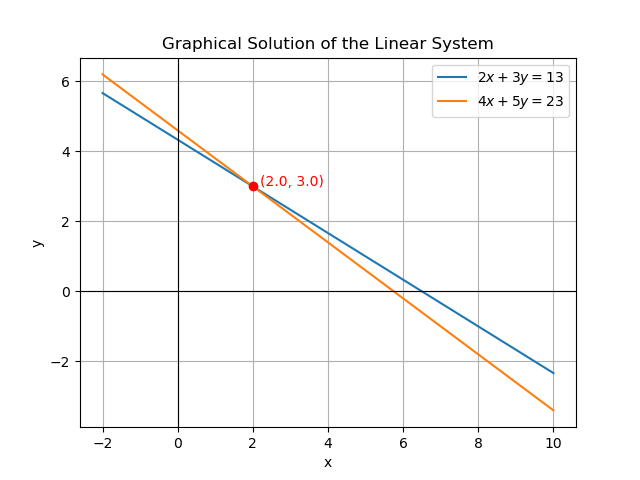
\includegraphics[width=0.8\columnwidth]{figs/fig.png}
     \label{fig:1}
 \end{figure}


\end{document}
